% Mirror: https://github.com/SIGma-UIUC/presentation-format
% --------------------------------------------------------------------
% This is a simple Beamer document. The shared styles live in ../sty/,
% Reading the comments should help you create a presentation even if
% you've never used Beamer before.
% --------------------------------------------------------------------

% Set our document class to Beamer
\documentclass[aspectratio=169]{beamer}
% Add handout option to collapse pauses for printing
% \documentclass[aspectratio=169, handout]{beamer}

% Presentation mechanics, then the SIGma look on top of them
\usepackage{../sty/slides}
\usepackage{../sty/sigma/sigma}

% Maths macros and algorithm environments
\usepackage{../sty/math}
\usepackage{../sty/stat}
\usepackage{../sty/algo}
\usepackage{../sty/code}

\usepackage{tikz}
\usetikzlibrary{graphs}
\usetikzlibrary{arrows.meta}

\usepackage{pdfpages}

% Set a title
\title{Lawn Mowing: special cases}

% Set a subtitle if you desire
% \subtitle{The traveling salesman and more}

% Whoever worked on the presentation:
\author{Ian Chen, Mihir Tandon}

% Date looks ugly, so leave blank
\date{}

% An institute name, if you're so inclined
% \institute{University of Illinois Urbana-Champaign}
% --------------------------------------------------------------------

% Begin document
\begin{document}

% Beamer calls each slide a "frame", defined within the environment:
% \begin{frame}
%   <frame content here>
% \end{frame}

% This frame is just the title.
\begin{frame}
    \titlepage
\end{frame}

\begin{frame}{Lawn Mowing and Milling}
    \begin{itemize}
        \item Given a \emph{lawn} $L \subset \Z^2$, and $k$ robots $R \subset \Z^2$ $\ldots$
        \item find $k$ tours $\tau_1, \ldots, \tau_k$ such that $\ldots$
              \begin{itemize}
                  \item $\cup_{i=1}^k (\tau_i + R) = L$ (milling)
                  \item $\cup_{i=1}^k (\tau_i + R) \supset L$ (mowing)
              \end{itemize}
        \item minimizing $\max_{i=1}^k \abs{\tau_i}$
    \end{itemize}
\end{frame}

\begin{frame}{Rectangles and rectangles}
    \begin{itemize}
        \item Suppose the lawn is an $M \times N$ rectangle, we have $k=1$ robots, shaped as an $m \times n$ rectangle\footnote{assume $m \ge n$ WLOG}.
    \end{itemize}
\end{frame}

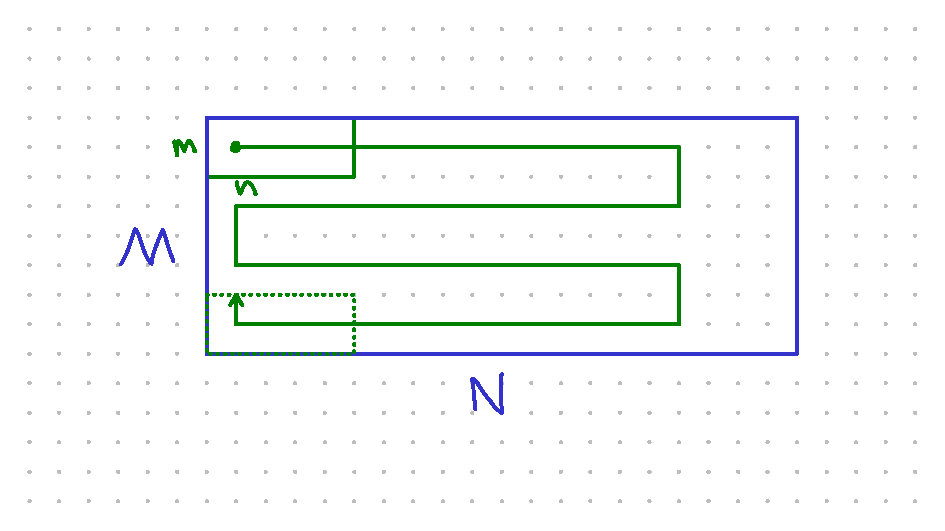
\includepdf[pages=-]{figs/snake.pdf}

\begin{frame}{An additive approximation:}
    \begin{itemize}
        \item Path length:
              $$
                  L \le \underbrace{(N - n)}_{\text{vertical length}} \times \underbrace{(\ceil{M/m} + 1)}_{\text{number vertical passes}} + \underbrace{2(M - m)}_{\text{horizonal moves}}
              $$
        \item Each robot step visits at most $m$ new grid locations
        \item $m \times \texttt{OPT} + mn \ge MN \implies \texttt{OPT} \ge MN / m - n$
        \item Thus, $L - \texttt{OPT}$ is bounded:
              $$
                  L - \texttt{OPT} \le \ab( (N - n) \times (M/m + 2) + 2(M - m) ) - \ab( MN / m - n ) \le 2(M+N)
              $$
    \end{itemize}
\end{frame}

\begin{frame}{More special cases}
    \begin{itemize}
        \item Given $k$ rectangular robots and an arbitrarily shaped lawn, can we find good solutions?
        \item Given $k$ arbitrarily shaped robots and a rectangular lawn, can we find good solution?
    \end{itemize}
\end{frame}

\end{document}
